\chapter{Introduction}

Production of x86 platform processors started big frequency competition.
Manufacturers have been releasing processors with more and more higher operating frequency.
Behind this competition has been research of a new production technologies that allows to integrate more transistors onto smaller area.
Gradually manufacturers started to realize that it is impossible to continue this frequency race forever.
More computing units started to be integrated into a single processor.
This first among common desktop processors was Intel's Pentium\textsuperscript{\textregistered} with hyper threading.
This processor was able to execute two threads at a time.
Since then quick boom of multi-core integration started even among other big processor manufacturers.
Integration of more execution cores allows less power consumption.
This factor is nowadays especially important due to processor integration into laptops and even due to environmental issues.
That's why current effort of processor manufacturers is to gain the best performance to power consumption ratio.

General purpose cores are integrated into the current common processors.
This means they have a pipeline for instruction execution with several stages.
Instruction can be in several states in such a pipeline, e.g. fetched, awaiting operands, ready, executed.
Instruction does not flow among the stages in the order that designates the program but the order is decided by the processor itself.
The decision is based on variety factors and predictions.
One of the pipeline stages is branch-prediction unit that has to predict the most probable flow of the executed program.
When this prediction is false whole pipeline has to be discarded and execution of the right branch of the program has to be started.
Processors suffer heavily from these mispredictions because it leads into big execution holes in which the processor pipeline stalls or is being reset.

Cache misses are another general purpose processor suffering.
Cache miss occurs when requested data are not within processor cache and have to be loaded from memory.

Although many improvements were implemented into the general purpose processors they still suffer from the described problems.
This is one of the reasons why collaboration of three big companies IBM, Sony, and Toshiba started development of Cell B.E. processor.
Processor that is multi-core, has good performance to power consumption ratio and is able to overcome the problems that the general purpose processors suffer.
That is because it allows the programmer to somewhat manage processor cache and branch prediction unit.

\chapter{Cell B.E. platform}

This chapter will introduce Cell Broadband Engine processor (Cell B.E.), the whole platform and its specific details.
The particular Cell B.E. processor will be described and illustrated.

\par
Cell B.E. processor is representative of a new generation of IBM's Cell B.E. platform family.
Cell B.E. is an asymmetric, high-performance multi-core processor that combines eight synergistic processing elements (SPE) and a Power Processing Element (PPE), which is a general-purpose IBM Power PC\textsuperscript{\textregistered} core.
Next part is a central memory element.
PPE can operate with the central memory directly while SPE indirectly, see below.
In Cell B.E. there are several kinds of memories.
All the elements are connected through high speed bus (EIB - Element Interconnect Bus).
Whole layout is on the figure \ref{fg:processorLayout}.

\begin{figure}
    \centering
    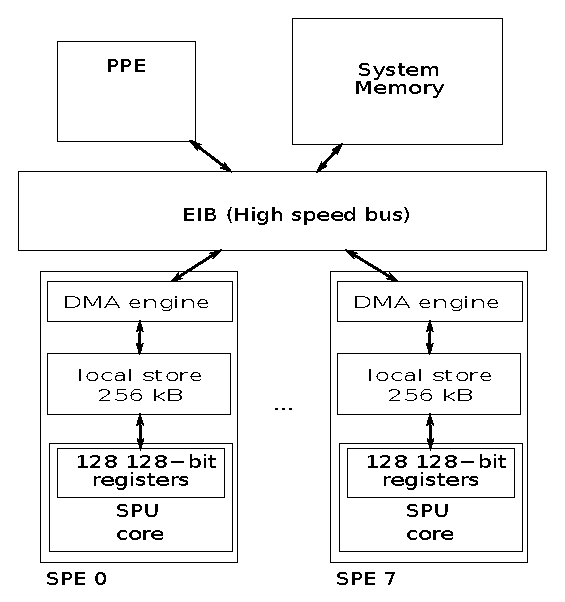
\includegraphics[width=0.7\textwidth]{data/cellLayout}
    \caption[Cell B.E. processor layout]{One PPE unit along with eight SPE stream processor units and system memory connected together with high speed EIB bus}
    \label{fg:processorLayout}
\end{figure}

Cell B.E. achieves a significant performance per Watt and performance per chip area advantage over conventional high-performance processors.
Is significantly more flexible and programmable than single-function and other optimized processors such as graphics processors, or conventional digital signal processors.
While a conventional microprocessor may deliver about 20+GFlops of single-precision (32b) floating-point performance, Cell delivers 200+ GFlops (in ideal conditions) at comparable power.

A number of signal processing and media applications have been implemented on the Cell B.E. with excellent results.
Advanced visualization such as ray-casting, ray-tracing, and volume rendering.
Or streaming applications such as media encoders, decoders or encryption and decryption standards have also been demonstrated to perform about an order of magnitude better than conventional PC.


\section{PPE - Power Processing Element}
PPE is derived from IBM Power PC\textsuperscript{\textregistered} core. Has 512kB L2 on die cache.
It supports the Power Architecture ISA, inherits the memory translation, protection, and SMP coherence model of mainstream 64-bit Power processors.
Virtualization (logical partitioning), large pages, and other recent innovations in the Power architecture are supported as well.
Programming for the PPE is the same as for conventional processors due to direct access to central memory.

\section{SPE - Synergistic Processing Element}

\par
SPE is an autonomous processor (sometimes called accelerator) targeted for computational intensive applications.
Each SPE has a SIMD core (SPU), a high-speed private local store memory and a direct memory access (DMA) engine.
The SPU unit has 128 128-bit wide unified general purpose registers to store all types of data.
It supports a SIMD-RISC instruction set.
It contrasts with traditional RISC processors where registers are divided according data types.
SPU has two pipelines, the odd one and the even one, so it can execute two instructions at a time (dual-issue) if few conditions are met.
Vectorized operations in various data types configurations can be performed with these registers e.g. two double-precision floats or eight 32bit integers can be processed at single clock tick.

\par
Unlike conventional microprocessors, SPE does not have a hardware cache.
Its function supply the small on-chip local store memory under programmer's control.
This allow code optimizations that can reduce cache misses.
The local store is separated from the main memory (on which the PPE operates), so SPE has its own address space.
Therefore any synchronization with other cores is not necessary.
The local store is attached to a larger (central) shared memory through DMA engine that manages transferring data from central memory to local store and vice versa as well as between two local stores.
We say that data is "DMAed" from source to destination.
DMA commands can be issued in many ways like in synchronous, asynchronous or in scatter-gather manner through DMA lists.
Therefore the Cell B.E. processor can be viewed as a distributed memory multiprocessor.
This memory management is another big part of programming for the Cell B.E.

\par
Programming for SPE has is a bit different compared to programming for a conventional processor.
Programmer have always to count with the fact that he has only 256kB for the program and data.

\par
This processor is embeded in Sony Playstation 3 (PS3, figure \ref{fg:cellmachines} a) game console as well as IBM Blade servers (figure \ref{fg:cellmachines}b ) where two processors on one board, building block.
There can be more boards connected in one system which creates powerfull and modular machine.
We have two PS3 machines available for this work.

\begin{figure}
    \centering
    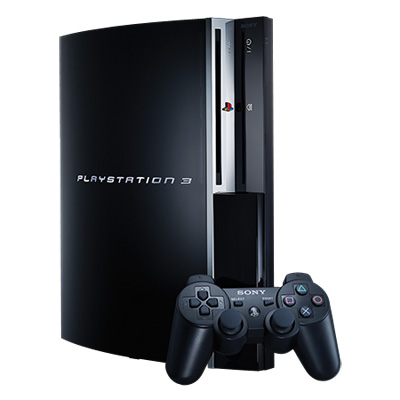
\includegraphics[width=0.3\textwidth]{data/png/PS3}
    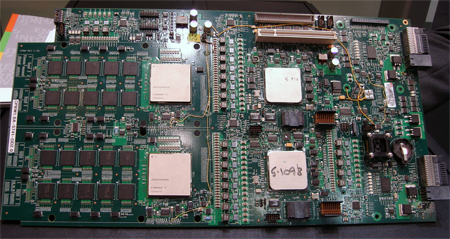
\includegraphics[width=0.6\textwidth]{data/png/ibm-cell-board}
    \caption[Cell B.E. based machines]{Images of Cell B.E. based machines
    \textbf{a)} Sony's Play Station 3 (image taken from www.boygeniusreport.com)
    \textbf{b)} IMB Cell Blade board (image taken from www.ps3tester.com)
}
    \label{fg:cellmachines}
\end{figure}

